For our initial design, we restricted the problem of re-randomization to only kernel modules. The argument here is that most of the kernel code (i.e., most of the device drivers, kernel libraries, etc) can be compiled as modules and the size of the core kernel can be reduced to the bare minimum. Possibility of JIT-ROP attacks on the core kernel can be minimized by scrutinizing the kernel code, ensuring that it is free of any memory disclosure vulnerabilities.
The kernel still uses KASLR -- the kernel image is loaded at a random address at boot time but is not re-randomized subsequently. The distribution and availability of ROP-gadgets across the kernel and its modules is analyzed in Section~\ref{se:eval_security}.

In the following sections, we describe how we implement efficient run-time re-randomization of the kernel modules. We describe how a module is logically split to aid re-randomization. The algorithm for stack and module re-randomization is also discussed in detail.

\section{Module Organization}\label{se:module_organization}
Every re-randomizable kernel module is split into two logical parts: \textit{movable} and \textit{immovable}. The movable part contains all of the code and most of the data, and the immovable part contains glue code (function wrappers) and some data (that need to be stored with the kernel). During re-randomization only the movable part of the kernel is relocated to a new address space while the immovable part remains static. Since the immovable part does not contain any module functionality and is never moved, it can be thought of as an integral part of the kernel. In Figure~\ref{fig:design}, we show a typical module layout.

\begin{figure}[ht!]
\centering
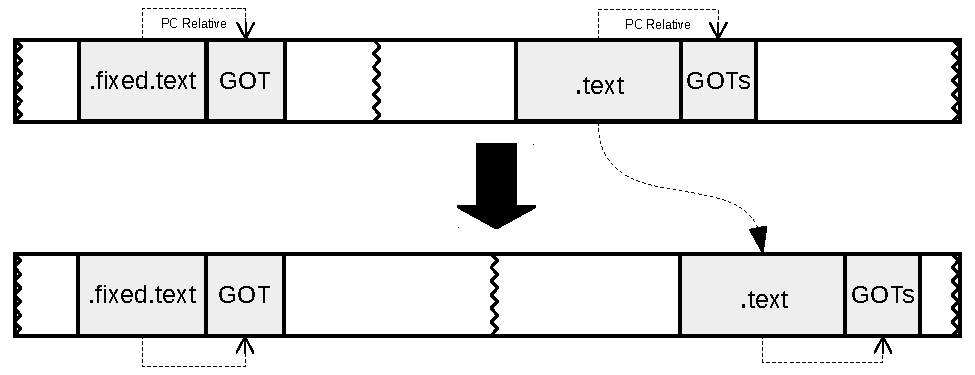
\includegraphics[width=.8\columnwidth]{pictures/rand_got.pdf}
\caption{GOT}
\label{fig:gots}
\end{figure}

\begin{figure}[ht!]
\centering
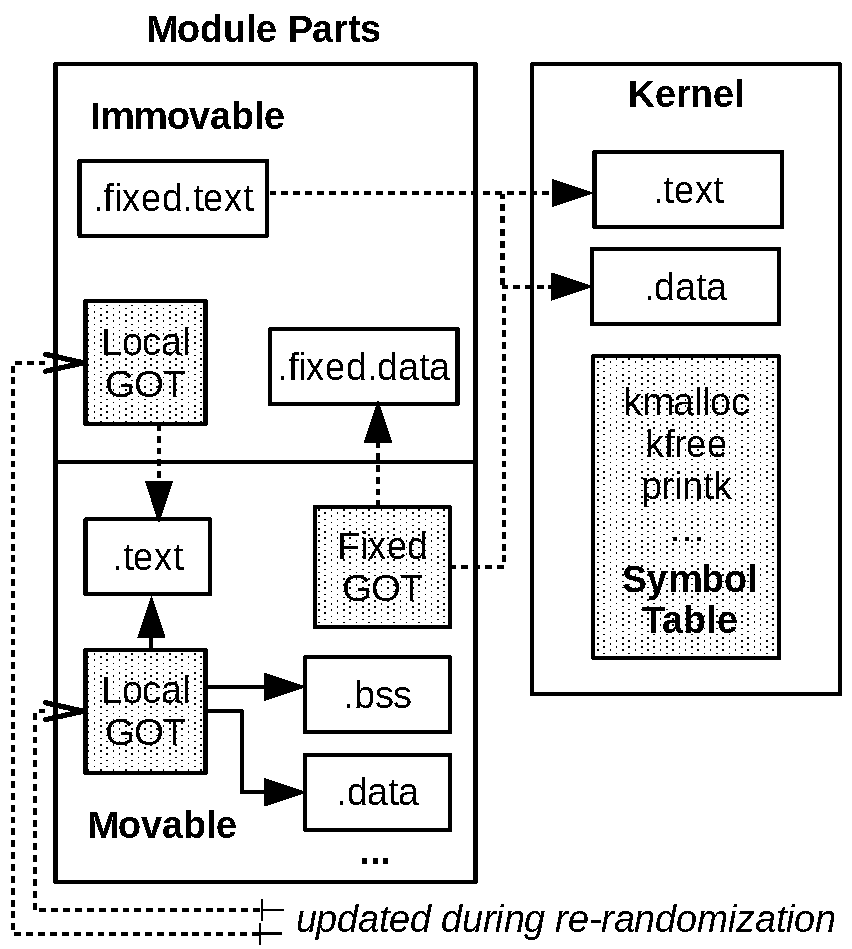
\includegraphics[width=.6\columnwidth]{pictures/design.pdf}
\caption{Design of re-randomizable modules~\cite{Adelie}}
\label{fig:design}
\end{figure}

The immovable and movable parts of the module can be placed anywhere in the 64-bit address space but due to ISA limitations, GOTs need to be within $\pm 2$GB of the code where they are accessed. This restriction arises from the fact that GOT entries are accessed using PC relative addressing which imposes a limitation on the distance between the table and the code that accesses it. This is why we need to maintain separate GOT tables for each part of the module.

A GOT table may contain two types of symbols: static and non-static (randomized) symbols. Static symbols, like global kernel references, do not need to be updated at the time of randomization while randomized symbols, like module-local symbols, are updated during randomization. To easily identify and update all the non-static symbols in the module, we create two GOTs. \textit{Fixed GOT}, that contains all the static symbols and \textit{Local GOT}, that contains all the symbols that need to be updated on re-randomization.

The movable part of the module contains both GOTs while the immovable part of the module only contains \textit{Local GOT}. As this part comprises only of thin function wrappers written entirely in assembly, the need for \textit{Fixed GOT} is avoided by directly having the 64-bit address of fixed functions in the code.

\section{Zero-copy Address Re-Map}
A major novel aspect of our work is that, unlike Shuffler~\cite{SHUFFLER}, we completely avoid copying of code and static data while re-randomizing addresses.
In Figure~\ref{fig:architecture}, we demonstrate the high-level principle.
Initially, at instant 1, both the kernel and the modules are in some randomly chosen address space, any distance apart from each other. This is achieved using our extended 64-bit KASLR. Periodically, module locations are re-randomized by a special \textit{randomizer} kernel thread. This thread creates new mappings, as shown at instant 2. Finally, when old regions are no longer used, we unmap them. In this process, no copying is actually made; we simply create a new page table entries that point to the same physical memory location.

\begin{figure}[ht!]
\centering
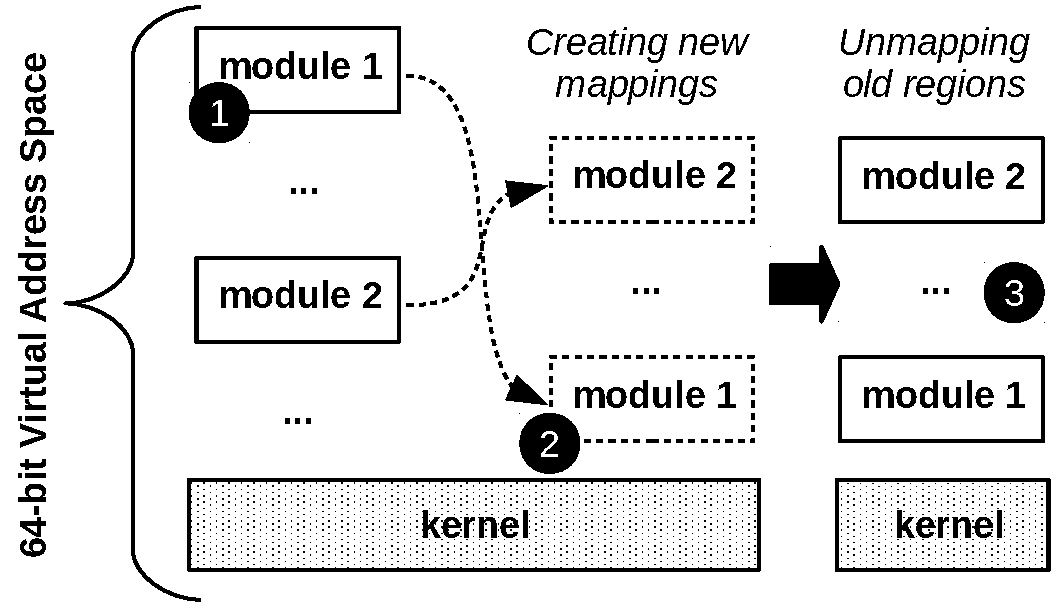
\includegraphics[width=0.7\columnwidth]{pictures/architecture.pdf}
\caption{Zero-copy mechanism~\cite{Adelie}}
\label{fig:architecture}
\end{figure}

\section{Controlling Address Space Lifetime}
It is crucial to timely delete old code from the memory, so that gadget addresses quickly become obsolete and useless for an attacker. Techniques used today (e.g., in Shuffler~\cite{SHUFFLER}) involve making a new copy of code, pausing threads, and unwinding the stacks. Previous code copy is removed after all the threads are done unwinding and updating the symbols on their corresponding stacks. While these techniques work in user space, kernel code is quite complex and functions can be called through long chains eventually leading to some user space thread making a system call. Due to low latency requirements of operating systems, the approaches that require pausing execution are infeasible and impractical to be used in the kernel space.

Our solution to this problem is to use deferred unmapping. The main idea
is to let pending calls finish execution in the old virtual address space. All function calls post re-randomization execute in a new virtual address space. Both old and new virtual address spaces map to the same physical pages, making simultaneous execution possible. As soon as the last pending call completes, the previous address range is immediately unmapped. Since almost all
kernel space calls should be relatively quick (or, otherwise it 
would indicate some bug in the code), the old pages do not stay mapped in memory long enough to be useful to an attacker.

The main challenge in effective address space lifetime management is to keep track of pending calls with little
overhead and in a scalable manner. Although the technique of reference counting~\cite{LFRC} used in memory reclamation can solve this problem, it can be slow in multi-core systems where updating a global
reference counter creates a hotspot for multiple CPUs. Instead,
we use the Hyaline lock-free memory reclamation~\cite{nikolaev2019hyaline}, which largely solves the same problem of efficient, optimistic memory access to blocks that are concurrently being deallocated by other threads. The main idea of the approach is to enclose operations that access potentially disappearing memory blocks with |mr_start()| and |mr_finish()|.
These special operations postpone memory reclamation until after all pending calls (i.e., those that
called |mr_start|) execute |mr_finish()|.
In this model, memory blocks are not de-allocated directly, instead, they are first \textit{retired} with
a special |mr_retire| operation. Only after pending calls from all threads complete, does the de-allocation take place. We refer the reader to~\cite{nikolaev2019hyaline} for more details regarding the Hyaline lock-free memory reclamation.

\section{Function Wrapping}
\label{se:function_wrapping}
One crucial step for making a module randomizable is wrapping all of its externally accessible functions. Any module functions that can be called by rest of the kernel must be wrapped for three reasons:

- First, this allows module address space to be re-randomized without breaking any function pointers that the kernel may hold. Module functions are not directly exposed to the kernel. Instead, all the external functions are wrapped with a thin wrapper, and the reference to the wrapper is passed to the kernel. By placing the wrapper function in the fixed part of the module, the movable part of the module can be freely moved in the memory whilst still maintaining valid kernel pointers. At the time of re-randomization, the function wrappers must be patched to point to the new location of the module, as discussed in detail in Section~\ref{se:module_randomization}.

One might argue against the indirection introduced by function wrappers and suggest directly updating the kernel pointers after re-randomization. This raises certain challenges. The pointer passed to kernel may propagate, in which case, all the pointers must be tracked and updated. Certainly there exist previous works on pointer tracking. However due to the Linux kernel's non-standard use of pointers\footnote{Pointers are sometimes used in kernel in non-standard ways. For example, LSB of pointers is sometimes used for a flag. Hence pointers can not be directly and automatically updated without considering the context of each individual pointer.} \cite{Linux_Pointer_NON_STD} this problem becomes intractable.

- Second, wrapping all the entry points to the module provides an easy way to control its address space lifetime using memory reclamation.

- Third, wrapping functions allows for the module's stack to be randomized. Stack randomization is discussed in Section~\ref{se:stack_randomization}.

Listing \ref{lst:before_wrapping} and \ref{lst:after_wrapping} give a high level overview of how a function wrapper works. The original function named \verb|func| is renamed to \verb|func_real| and a wrapper function with the name of \verb|func| is created that calls the actual implementation \verb|func_real|. The rest of the module keeps using the name \verb|func| in its code.

\lstset{language=C}
\begin{lstlisting}[frame=single, caption={Original Function},label={lst:before_wrapping}]
long func(long arg)
{
    // code
}

kernel_ref(&func);
\end{lstlisting}

\lstset{language=C}
\begin{lstlisting}[frame=single, caption={Wrapped Function},label={lst:after_wrapping}]
/* Movable function */
long func_real(long arg)
{
    // code
}

/* Fixed function */
long func(long arg)
{
    mr_start();
    randomize_stack();
    long ret = func_real(arg);
    restore_stack();
    mr_finish();
    return ret;
}

kernel_ref(&func);
\end{lstlisting}

\subsection{Naked Wrapper}
The function wrappers are implemented as \verb|naked| functions. A naked function is a special function for which the compiler does not generate any prologue or epilogue. These functions can only contain assembly instructions. Naked functions are used instead of pure assembly functions to take advantage of compiler type checking. Writing the wrapper function in the assembly has two advantages. Firstly, it allows for freedom of doing non-conventional things like randomizing the stack of a running program. Secondly, wrapper function could be made really thin by explicitly avoiding calls through PLT or GOT.

In x86-64, the first six arguments to a function are passed through registers. At the entry point of the wrapper, registers |rdi|, |rsi|, |rdx|, |rcx|, |r8| and |r9| contain the arguments for the wrapped function. However, before the wrapped function is called, we need to call other functions such as |mr_start()| and |randomize_stack()|. Calling these functions before the wrapped function could clobber the registers, destroying any arguments passed by the caller. Similarly, function's return value is also returned through a register. Thus the return value of the wrapped function could also be destroyed by subsequent calls to |mr_finish()| and |restore_stack()|. The registers must, therefore, be carefully handled to ensure the preservation of the arguments and return value of the wrapped function. In our implementation of the wrapper, we follow the x86-64 ABI for function calls. We push all the volatile registers containing arguments for the wrapped function onto the stack at the beginning of the wrapper. The registers are then restored before the wrapped function is called. Wrapped function's return value is also similarly saved and restored. The pseudo-code for the naked wrapper function is described in Listing~\ref{lst:naked_wrapper}.

\lstset{}
\begin{lstlisting}[frame=single, caption={Naked Wrapper Function},label={lst:naked_wrapper}]
Save base pointer
  Push arguments to the stack
    Call mr_start() and randomize_stack()
  Pop arguments from the stack
  Call wrapped_function()
  Save return value
    Call mr_finish() and restore_stack()
  Restore return value
Restore base pointer
\end{lstlisting}

\section{Data Wrapping} \label{se:data_wrapping}
Similar to function wrapping, all the structs and variables passed to the kernel must be wrapped as well. The kernel could keep a reference to any data structure passed to it. These data structures must hence be placed in the fixed part of the module. Placing them in fixed sections keeps the kernel references valid while the movable part of the modules is relocated to a new address space. Section placement is achieved  by using the \verb|section| attribute of GCC compiler. The variables are placed in the \verb|.fixed.data| section and constants are placed in \verb|.fixed.rodata|. During re-randomization, all the fixed sections are recognized by the |.fixed| prefix in their section names and are left as is.

\section{Stack Randomization}
\label{se:stack_randomization}
Randomizing stack is not a trivial task. Linux kernel maintains multiple stacks for each task. Each thread needs its own stack and the stack randomization process needs to be fast. Device drivers typically have many interrupts registered. Interrupt handlers run asynchronously, preempting other tasks and interrupt handlers. While an interrupt is being served other interrupts in the systems may also be disabled. Any delays in the top half of the interrupt service routine can have severe repercussions. Therefore it is really important to have a fast stack swapping methodology.

Our approach is to maintain a per-CPU lock-free (LIFO) list of stacks. We randomize the stack at the beginning of the function wrapper by dequeuing the head of the per-CPU list. Old \verb|%rsp| is saved in the \verb|%rbp| and \verb|%rsp| is replaced with the newly dequeued stack. Before exiting the wrapper the stack is returned to the head of the queue and \verb|%rsp| is restored from \verb|%rbp|.

The LIFO implementation of the list provides good temporal locality. High frequency interrupts grab and release the same stack, this ensures that the cache is always hot and causes minimal thrashing. Moreover, since a different list is implemented for each CPU the contention is low and high performance is achieved.

For performance reasons, the anticipated number of stacks are eagerly allocated and kept in the LIFO list. Eager allocation of stacks prevents costly \verb|kmalloc| calls in the wrapper functions. Through experiments we found that five stacks for each CPU are enough for most purposes, although in rare cases when more stacks are needed, they will be dynamically allocated as shown in Listing~\ref{lst:get_stack}.

In the head of the list we keep a \verb|version| field, this field is used to prevent the old stacks from being reused after re-randomization. At the time of randomization we create a new per-CPU list of stacks with incremented $version$. The old lists are replaced by new ones by a \verb|CAS| operation. All the elements on the old list are emptied into per-CPU \verb|trash list|. At this point, all the old stacks that are currently not checked-out are taken out of circulation. To avoid putting the old stacks back into the list, whenever a stack is returned, its \verb|version| is checked. If it does not match the \verb|version| of the list head, it is put into \verb|trash list| instead of the LIFO list. It is important to note that even though all the stacks are removed from the LIFO list, it is not safe to free them just yet. This is because a sleeping thread which is in the process of dequeuing a new stack from the LIFO list may still hold a reference to it. We have to wait till all the threads have left the address space of the module and it is safe to reclaim memory. The |trash lists| are then traversed and all the old stacks are freed.

x86-64 accepts the first six function arguments through the registers and any additional arguments are passed on the stack \cite{X86_ABI}. In our work, we did not discover any function calls with more than six arguments, so we simply replace the stack pointer to point to the new randomized stack. Any local variables passed by reference will remain on the old stack and the pointer arguments will keep pointing to them. This implementation avoids the lengthy process of stack unwinding and copying, and allows us to keep stack swapping logic minimal. All the functions executed from the untrusted module, however, will use the new randomized stack.

\lstset{language=C}
\begin{lstlisting}[frame=single, caption={Stack Randomization},label={lst:stack_randomization}]
%rbp = %rsp;
%rsp = get_stack();
...
return_stack(%rsp);
%rsp = %rbp;
\end{lstlisting}

\lstset{language=C}
\begin{lstlisting}[frame=single, caption={get\_stack()},label={lst:get_stack}]
void *get_stack()
{
    void *stack = pop_stack_this_cpu();
    if (stack == NULL)
        stack = allocate_stack();
    return stack;
}
\end{lstlisting}

\lstset{language=C}
\begin{lstlisting}[frame=single, caption={return\_stack()},label={lst:return_stack}]
void return_stack(void *stack)
{
    push_stack_this_cpu(stack);
}
\end{lstlisting}

The lock-free LIFO list implementation is standard and is not documented in this report. The only deviation from the standard is that we have used some bits of the $aba\ stamp$ word to track the $version$ and $size$ of the stack, see Listing \ref{lst:stack_head}. x86-64 only supports 128-bit compare-and-swap ($CAS$) operations, 64 bits are required to store the pointer to the head node, the remaining 64 bits are usually used to store the aba stamp. Since our head must fit in 128 bits for $CAS$ operation, in our implementation we used bit-fields to split the 64 bit word into aba, version, and size. For practical purposes, a 48-bit aba stamp is enough to solve the ``ABA problem''~\cite{CAS_Reactor}.

\lstset{language=C}
\begin{lstlisting}[frame=single, caption={Head Structure},label={lst:stack_head}]
struct head {
	struct stack_node *head;
	union {
		struct {
			u64 size:8;
			u64 ver:8;
			u64 aba:48;
		};
		u64 stamp;
	};
} __aligned(16);
\end{lstlisting}

\section{Module Re-Randomization}
\label{se:module_randomization}
The process of loading a module is different for re-randomizable and non-re-randomizable modules. Vanilla Linux allocates the module in two chunks, \textit{init} \verb|module_layout| containing the module initialization code and \textit{core} \verb|module_layout| containing the core functionality of the module. For re-randomizable modules, we create an additional \textit{fixed} \verb|module_layout| for the fixed part of the module. For a re-randomizable module, all the sections that are identified to be fixed are allocated in the \textit{fixed} layout at load time.

In vanilla Linux, once the module is done loading, all the artifacts that are no longer required are freed. Specifically, relocation and symbol tables are deallocated from the memory. However, since we need to patch the binary again each time it is randomized, we save the relocation and the symbol tables.

Reapplying relocations is a costly process, we are mindful to only keep the relocations that are required. Under the position-independent code, most of the relocations are not required to be reapplied and can be gotten rid of. We remove all the relocations of the following types:
\begin{verbatim}
R_X86_64_PC32,
R_X86_64_PC64,
R_X86_64_REX_GOTPCRELX,
R_X86_64_GOTPCRELX,
R_X86_64_GOTPCREL,
R_X86_64_PLT32
\end{verbatim}
Furthermore, we also remove the relocations of type \verb|R_X86_64_64| that reference fixed symbols.

For re-randomizable modules, we have three GOTs instead of one. Based on section (fixed vs. movable parts) and symbol locality, we choose one of those tables when generating a corresponding entry. Occasionally, two tables will contain duplicates of the same symbol (e.g., a local GOT entry
from the immovable part can point to the same address as a local GOT entry from the movable part). We use separate GOTs for movable and fixed parts because these parts can be any distance away from each other, while GOTs must always be placed within $\pm 2$GB reach from \%rip due to the ``RIP-relative'' address mode, as discussed in detail in Section~\ref{se:module_organization}.

During module re-randomization, the randomizer kernel thread periodically performs the following steps:
\begin{enumerate}
\item A new virtual address space map is created that maps to the same physical addresses as an old map. This mitigates the need of copying the module code and data.

\item The addresses of the randomized symbols in the symbol table are updated. This symbol table is subsequently used to reapply the relocations.

\item Randomized symbols in the movable GOT are updated.

\item The module is patched by reapplying the required relocations.

\item A custom function is called from the module to update its run-time function pointers. This is only required for some modules that use run-time function pointers.

\item Randomized symbols in the fixed GOT are updated. This GOT is what is used by the wrapper functions to jump to the real function implementations. Updating this table migrates the execution from the old address space to the new address space.

\item \textit{mr\_retire()} is called from the memory reclamation algorithm to request unmapping of the old address space.
\end{enumerate}
After that, the randomizer thread sleeps for the specified re-randomization period and then repeats the entire process.
The memory reclamation algorithm asynchronously unmaps the previous address space when all pending calls complete and it is safe to unmap.